\chapter{Our work}
\label{kap:kap3}

In this chapter, we shall look into our proposed enhancements to the existing
implementations of RRR. Firstly, we propose a new block encoding method.
Then, we show how we can exploit the assumptions about the share of ones
in the bit sequence.

\section{Block encoding}

As we already discussed in section~\ref{section:compressed_bv}, there are to
the best of our knowledge two widely used methods to encode and decode the
blocks in RRR. The main disadvantage of the table decoding method is the big space
overhead that it poses and the inability to reasonably support longer blocks
in practice because of the huge table sizes for bigger block length. On the
other hand, the on-the-fly decoding method may be used to support a bigger block size
with the downside being longer encoding and decoding times. We propose
new method of encoding and decoding the blocks. The main objective of the new method is
to create an alternative to the previous methods that enables use of longer blocks
while not hurting the runtime so significantly.

The main idea behind our solution is to use a divide-and-conquer approach to break
the problem of finding the order of the block $B$ along the class $c$ to finding the order
of the several smaller blocks. This may for example enable us to use the table method to solve the
smaller subproblems. To facilitate our solution, we need to alter the respective order of
the blocks along the same class. We want to note that we also use the number of ones to
identify the class of block. However, both previous solutions used the lexicographical ordering
for the blocks that shared the same class. In our solution, every block $B$ will be thought
of as two smaller blocks of half the size, namely $B_1$ and $B_2$. We shall at first sort the
big block $B$ by the pair $(c_1, c_2)$ where $c_1$ and $c_2$ are the respective classes of the
smaller blocks $B_1$ and $B_2$. Only then, we break the ties by lexicographical order of $B_1$ and $B_2$.
Note that the original lexicographical ordering can be rephrased in the context of sub-blocks as sorting
at first by $B_1$ and then by $B_2$. The example of the ordering for concrete block length
and class is shown on Figure~\ref{obr:lexicographicalVsUs}.

\begin{figure}
	\centerline{
        \begin{tabular}{l c l}
            Offset  &   Block       & $(c_1, c_2)$\\
        \hline
            \small 0&   \tt 000 011 & \multirow{3}{*}{$(0, 2)$}\\
            \small 1&   \tt 000 101 & \\
            \small 2&   \tt 000 110 & \\
        \hline
            \small 3&   \tt 001 001 & \multirow{5}{*}{$(1, 1)$}\\
            \small 4&   \tt 001 010 &\\
            \small 5&   \tt 001 100 &\\
            \small 6&   \tt 010 001 &\\
            \small 7&   \tt 010 010 &\\
        \end{tabular}
        \hspace{3em}
        \begin{tabular}{l c l}
            \small 8&   \tt 010 100 & \multirow{4}{*}{$(1, 1)$}\\
            \small 9&   \tt 100 001 &\\
            \small 10&  \tt 100 010 &\\
            \small 11&  \tt 100 100 & \\
        \hline
            \small 12&  \tt 011 000 & \multirow{3}{*}{$(2, 0)$}\\
            \small 13&  \tt 101 000 &\\
            \small 14&  \tt 110 000 &\\
        \end{tabular}
	}
	\caption[TODO]{
        Example of the new ordering for the block length $b=6$ and class $c=2$.
        Every block is divided into two sub-blocks of size 3. Note the differences to the
        lexicographical ordering. Block {\tt 011 000} on offset 12 is preceded by lexicographicaly
        greater blocks {\tt 100 001}, {\tt 100 010} and {\tt 100 100} as it has bigger number of ones
        in the first sub-block.
    }
	\label{obr:lexicographicalVsUs}
\end{figure}

We shall now demonstrate how we use this new ordering and that it is convenient to encode and
decode $B$ in a divide and conquer manner.

\paragraph{Encoding}

Before providing the general encoding stratedy, we shall demonstrate the encoding with
simple example and then generalize the ideas behind the process. Imagine encoding
block {\tt 100 010}. We can see that the class of this block is 2 as there are two ones in
the whole block. Obtaining the offset is more complicated. We will proceed by enumerating the
number of blocks preceding {\tt 100 010} in the class $c=2$. We divide the blocks preceding it
along its class into 3 categories:

\begin{itemize}
    \item Blocks with smaller number of ones in the first sub-block.
    (There are 3 such blocks -- those beginning with {\tt 000}.)
    \item Blocks with same number of ones in the first sub-block, but smaller first sub-block.
    (There are 6 blocks with this property -- those beginning with {\tt 010} or {\tt 001}.)
    \item Blocks with same first sub-block, but smaller second sub-block.
    (There is 1 such block, namely {\tt 100 001}.)
\end{itemize}

Summing up, we get that there are 10 blocks preceding {\tt 100 010} so it has the offset $o$
equal to 10. Together with class we would encode this block as a pair $(2, 10)$.

In general, consider a block $B$ of length $b$. The first step is to obtain
$c$ -- the class of the block. This can be done by counting ones in $B$. We
then get that $$c=\#_1(B)$$. To obtain the sequence number $o$ of $B$, we shall
count the number of blocks preceding $B$ along the class $c$. As we mentioned,
there are 3 types of blocks preceding $B$:

\begin{enumerate}
    \item Blocks with the first sub-block having smaller class than $B_1$.
    \label{chapter3:encoding:1}
    \item Blocks with the first sub-block being of the same class as is $B_1$
    but with smaller first sub-block. \label{chapter3:encoding:2}
    \item Blocks with the same first sub-block but smaller second sub-block.
    \label{chapter3:encoding:3}
\end{enumerate}

Formalizing this, we shall write $B\prec_X B'$ if blocks $B$ and $B'$ are of
the same length, class and $B$ precedes $B'$ in ordering $X$. We shall
write $B\prec_{\Lex} B'$ if $B$ preceeds $B'$ in lexicographical ordering.
To formally define our new proposed ordering $P$, we shall write that
\begin{align*}
    B\prec_P B' \iff
    &[\#_1(B_1) < \#_1(B_1')] \\
    &\lor [(\#_1(B_1) = \#_1(B_1')) \land B_1 \prec_{\Lex} B_1']\\
    &\lor [B_1 = B_1' \land B_2 \prec_{\Lex} B_2']
\end{align*}
where $B=B_1B_2$ and $B'=B_1'B_2'$.

The number of blocks in group~\ref{chapter3:encoding:1} is equal to
$$\sum_{i=0}^{c_1-1} {15\choose i} {15\choose c-i}$$ where $i$ denotes the number
of ones in the first block. Product of terms ${15\choose i}$ and ${15\choose c-i}$
denotes the number of blocks with $i$-ones in the first sub-block and the rest
$c-i$ ones in the second sub-block.

The number of blocks in group~\ref{chapter3:encoding:2} is equal to the number of blocks that
share classes of sub-blocks, but are smaller than $B$. Number of these blocks is $o_1\times {15\choose c_1}$.
The number of blocks in group~\ref{chapter3:encoding:3} is equal to the number of blocks smaller 
than $B_2$. This is identical to the offset $o_2$. Note, that to obtain the offset of $B$
we need the encoding of the blocks $B_1$ and $B_2$. These are two pairs of numbers
$(c_1, o_1)$ and $(c_2, o_2)$ that can be computed recursively.

\paragraph{Decoding}

Decoding is a process of obtaining block representation $B$ from the encoded
representation $(c, o)$. We would like to reuse the sub-routines for the blocks
of size $b/2$. However, to use these we need to find the classes and offsets of
the smaller sub-blocks. Namely, we need to find what the pairs $(c_1, o_1)$ and
$(c_2, o_2)$ are. This will be a 3 step process. We know that $c_1 + c_2 = c$.
All the possible blocks along the class $c$ are primarily sorted by pair $(c_1, c_2)$.
If we know what is the number of blocks that have the pair $(c_1, c_2)$ equal to
$(0, c), (1, c-1), \ldots , (c, 0)$, we can search using the offset in which of these groups
our block is located. This gives us classes of the sub-blocks $c_1$ and $c_2$. When we obtain
these two, we shall proceed to the second step. Along all the blocks that have the same $c_1$ and $c_2$,
we would like to find $o'$-th where the new offset $o'$ is given by subtracting the number of
blocks with the smaller pairs $(c_1, c_2)$, from the offset $o$. There are ${b/2 \choose c_1}$
and ${b/2 \choose c_2}$ ways how the first and second block may look respectively. As all the
possible combinations of first and second sub-block are possible, we want to identify $o'$-th block
along the ${b/2 \choose c_1}\cdot {b/2 \choose c_2}$ blocks. Blocks are sorted primarily
by the first sub-block and then by the second sub-block. This means, that the ordered sequence of
the blocks within class pair $(c_1, c_2)$ will be just all the possible ${b/2 \choose c_2}$
second sub-blocks repeating again and again, with the different, yet increasing
first sub-block. Furthermore, this cycle of ${b/2 \choose c_2}$ sub-blocks will repeat
${b/2 \choose c_1}$ times (once for each possible first sub-block). From $o'$ we can easily
find the order of the first and second sub-block. We just need to know how many cycles of length
${b/2 \choose c_2}$ happened until $o'$ and what is the offset of the second sub-block at which
the current cycle is on position $o'$. As the cycles are of the same length, this is straightforward.

% TODO: refactor from here

We shall again present this process on an example and decode the block from previous
encoding example {\tt 100 010} encoded as $(2, 10)$. To obtain the number of ones in
the first sub-block only from the offset of the block, we can look into the table and
see that there are 3 blocks with zero ones in the first sub-block. As the offset of our
block is ten, we need to look for this block between blocks with more than 0 ones. There
are 9 blocks with one 1 in the first sub-block. As $3+9$ is bigger than 10, we discovered
that the number of ones in the first block is 1 and it follows that the number of ones in
the second sub-block is
also 1 as we know the total number of ones in the block. There are 9 blocks with
this exact same property, the smallest one being {\tt 001 001} and largest one
{\tt 100 100}. We had successfully narrowed our search into these 9 blocks and can now
focus on identifying what is the offset of the first and second sub-block. There are
${3 \choose 1} = 3$ possibilities (namely {\tt 001}, {\tt 010}, {\tt 100}) how the first
and also the second block may look. Blocks are sorted according
to the first sub-block and then second sub-block. As all the combinations of the first
and second sub-block are possible, all possible second sub-blocks will be cyclically
repeating again and again with the increasing first sub-block. Cycle through
the sub-blocks will be of length 3 (number of possible second sub-blocks) and will repeat
3 times (number of possible first sub-blocks). Along these ordering of 9 blocks we are
looking for the 7th. From this, we know that the block, we are looking for contains a
first sub-block, that is along all the blocks of size 3 and class 1, third in the ordering.
So to find the first sub-block, we reuse the solution based on the lexicographical ordering
and ask it to decode pair $(1, 2)$ that gives us the first sub-block {\tt 100}. Obtaining
the second sub-block is not that hard. So far, we focused how many times the first sub-block
changes up to the 7th position. Now, we turn our attention on which second sub-block the cycle
ends. We know that every 3rd iteration, the second sub-blocks starts, where it began.

\paragraph{Combining encoding methods}

Our proposed method can be used to obtain the encoding and decoding scheme for block size $2b$
using only scheme for the block size of $b$. As we already mentioned in
subsection~\ref{subsection:block_size}, most of the implementations of RRR choose the size
of the block to be of form $2^k-1$ as the possible number of ones in the block is power of two and
its representation fits exactly into $k$ bits. This is not very convenient for us as combining two
solutions of size $2^k-1$ together gives us only solution for block size $2(2^k-1)$ what is one bit
short of a practically desired size $2^{k+1}-1$. To overcome this, we need to extend the block by one bit.
To do this, we shall once again alter the order of the blocks along the same class. Let us now look on
an example how to obtain blocks of length 5 and class 3. There will be two types of blocks
in this class. One of the form {\tt 0xxxx} and second of the form {\tt 1xxxx}. There are
${4\choose 3}$ ways how to distribute 3 ones along the four places so there will be exactly
4 blocks starting with 0 and ${4\choose 2}$ blocks starting with one. Blocks starting with
zero will continue with all the possible blocks of length 4 and class 3. These blocks can
come in any valid ordering but we can already use our newly devised technique of block
encoding. The complete order of the blocks in this example appears in Fig.~\ref{obr:bitExtension}.
\begin{figure}
	\centerline{
        \begin{tabular}{l c}
            Offset  &   Block      \\
        \hline
            \small 0&   \tt 0 0111 \\
            \small 1&   \tt 0 1011 \\
            \small 2&   \tt 0 1101 \\
            \small 3&   \tt 0 1110 \\
        \end{tabular}
        \hspace{4em}
        \begin{tabular}{l c}
            \small 4&   \tt 1 0011 \\
            \small 5&   \tt 1 0101 \\
            \small 6&   \tt 1 0110 \\
            \small 7&   \tt 1 1001 \\
            \small 8&   \tt 1 1010 \\
            \small 9&   \tt 1 1100 \\
        \end{tabular}
	}
	\caption[TODO]{
        Example of bit extension of block length 4 to length 5. Table shows the
        order of blocks along the class $c=3$. These are primarily sorted
        by the first expansion bit. Blocks with the same value of expansion
        bit are sorted according to the method we introduces previously.
    }
	\label{obr:bitExtension}
\end{figure}

We shall call this technique \textit{bit extension} technique. The fact that this
ordering can be encoded and decoded easily is based on the observation that this technique,
is just a generalization of our newly devised technique. Up to this point, we combined
scheme for the block size $b$ to obtain solution for block size $2b$. Combining method
for block size $b_1$ with method for block size $b_2$ yields the block size $b_1+b_2$
but uses the same arguments and ideas for encoding and decoding as we already presented. 

\section{Hybrid encoding}

% TODO: pridat viac kontextu, preco sa zaoberame percentami jednotiek
% TODO: ukazat ze vacsie b je lepsie

The main space saving in RRR happens in the way how the block is stored. If we have
a block of length $b$, then storing it in a raw bit representation takes $b$ bits.
Storing it in block compressed form depends on the blocks class. If the block
has class $c$ then compressed representation takes $\ceil{\log_2 (b+1)}$ bits to store the
class and $\ceil{\log_2{b\choose c}}$ to store the offset. In
Fig.~\ref{obr:rrrSpaceSavings} we can see for different block sizes how the space saved
per block depends on the blocks class. We can see RRR saves most of the memory on the
sparse blocks, those with small number of ones. Let us now consider a randomly
generated bit sequence $B$ of length $n$ containing $p\%$ of ones. We shall study how
often blocks with big number of ones arise in a sequence with small number of ones in it.

\begin{figure}
	\centerline{
		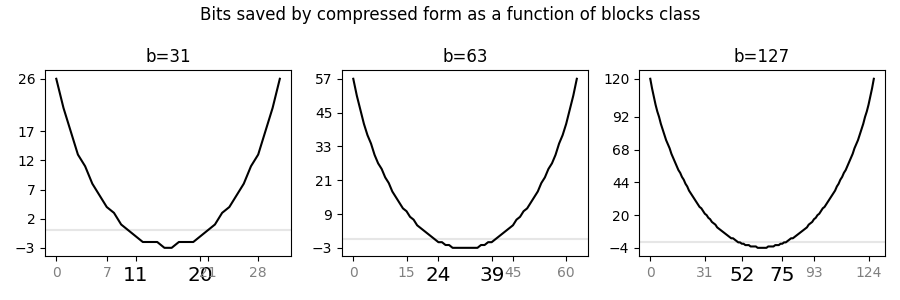
\includegraphics[width=\textwidth]{images/rrr_space_savings}
	}
	\caption[TODO]{Ratio of space used by the compressed
    block representation of blocks class and offset to the space used by storing the raw
    block. First, second and third graph represent how the ratio is dependent on the blocks
    class for 3 different block sizes 31, 63 and 127 respectively. Black numbers on the $x$-axis
    are denoting the start and the end of the interval where compressed version is even worse
    in the space usage (ratio over 1).
	}
    % can be found on https://github.com/Aj0SK/master-thesis/blob/main/text/images/rrr_space_savings.png
	\label{obr:rrrSpaceSavings}
\end{figure}

We shall make some general observations about the space distribution of block
classes of the random bit sequence containing $p\%$ of ones. If we consider a
block size $b$ then the random variable $X$ denoting number of ones in the
block follows a binomial distribution $$X \sim Bin(b,p).$$ As we can see in
Fig.~\ref{obr:hybridEncodingDistribution}, the probability of blocks
containing many ones in a sequence containing only 5\% of ones
decreases exponentially. Even in very long sequences, these blocks will
occur very rarely. This led us to a solution that we call a \textit{hybrid encoding}.

\begin{figure}
	\centerline{
		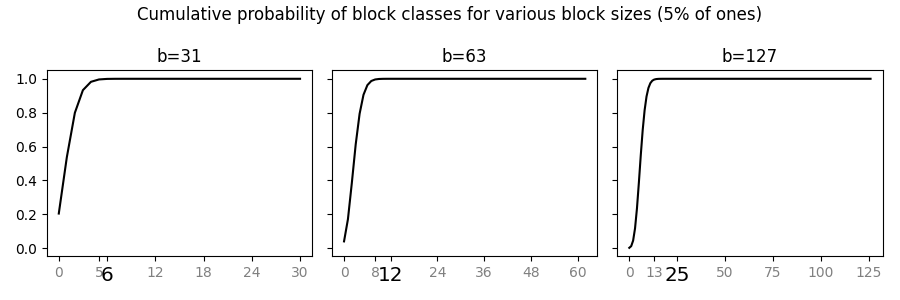
\includegraphics[width=\textwidth]{images/hybrid_encoding_motivation}
	}
	\caption[TODO]{On these 3 graphs, we can see the cumulative distribution
    of blocks classes for the block sizes of 31, 63, 127. The frequency of ones is
    fixed to 5\%. Note the marked classes on the $x$-axis. Numbers 6, 12 and
    25 mark the place up to which 99\% of probability distribution lies for
    the block sizes 31, 63 and 127 respectively.
	}
    % Can be found on https://github.com/Aj0SK/master-thesis/blob/main/text/images/hybrid_encoding_motivation.png
	\label{obr:hybridEncodingDistribution}
\end{figure}

Hybrid encoding uses a property that in some sequences blocks with high number
of ones are very rare. Encoding these blocks is not that helpful as their
compressed representation may take even more bits than the original raw
representation. Storing the whole block may waste memory if the number of
ones is big but there are not many possibilities how the block may look.
Although we shall waste some memory by this from time to time (for every
block that is almost completely filled with ones), we can save some small
amount of memory by decreasing the number of bits that we use to store
classes. The main idea of hybrid encoding is that every block with its
class bigger than some threshold will have its class set to this threshold
and this will mean that the block is stored using full $b$ bits instead of
$\ceil{\log_2{b\choose c_i}}$ bits. If we choose a $c_k$ as a value for cut off.
Blocks with bigger or equal class than $c_k$ will not be encoded but just
copied with the class set to $c_k$. Note that the class of the block
is a number from 0 to $b$. To possibly save some space on the bit representation
of the blocks class, we need to choose $c_k$ such that $\ceil{\log_2(c_k+1)} < \ceil{\log_2(b+1)}$.
We shall now compare these two representations and the theoretical space savings that
can be obtained. Let $n$ be a length of the sequence, $b$ the block size and $C_i$
number of blocks with class $i$. To simplify the calculation, we shall assume that $b+1$
as well as $c_k$ is a power of 2 and $n$ is divisible by $b$, also we shall
use $\lg x$ instead of $\log_2 x$. Using this notation, first representation is
consuming $$(n/b)\lg (b+1) + \sum_{i=0}^{b} C_i\ceil{\lg {b\choose i}}$$
bits of space with the first and second term being the number of bits that
is used by the classes and offsets respectively. The second representation
using the cutoff $c_k$ shall consume $$(n/b)\lg (c_k+1)+\sum_{i=0}^{c_k-1}C_i\ceil{\lg {b\choose i}} + \sum_{i=c_k}^{b}C_i b$$
bits of space. We would like to see what is the expected space that we save
using the hybrid encoding. We start by simplifying the expected value of the
difference of these representations:
% My mathematical guesswork
\begin{align*}
E[space] &= E\left[(n/b)(\lg(b+1)-\lg(c_k+1)) + \sum_{i=c_k}^{i\leq b}\ceil{C_i}\cdot \left(\ceil{{b\choose i}} - b\right)\right]\\
&=(n/b)(\lg(b+1)-\lg(c_k+1)) + \sum_{i=c_k}^{i\leq b}E\left[\ceil{C_i}\cdot \left(\ceil{{b\choose i}} - b\right)\right]\\
&=(n/b)(\lg(b+1)-\lg(c_k+1)) + \sum_{i=c_k}^{i\leq b}\ceil{E\left[C_i\right]}\cdot \left(\ceil{{b\choose i}} - b\right)\\
E[C_i] &= (n/b)\cdot {b\choose i}\cdot p^i\cdot (1-p)^{b-i}
\end{align*}

Here we used the linearity of the expected value. To compute the expected value of
$C_i$ we used the fact, that number of blocks of certain class follows binomial
distribution.

% some rough numbers from the program:
% https://github.com/Aj0SK/master-thesis/blob/main/code/experiment3/sdsl_theoretical_stat.py
% length of sequence, b, c_k, p     ->  classic vs hybrid and hybrid/classic
% For 31000, 31, 7, 0.05 the result is 11653 vs 9660 ... rate 0.83
% For 31000, 31, 15, 0.05 the result is 11653 vs 10653 ... rate 0.91
% For 63000, 63, 7, 0.05 the result is 21248 vs 19469 ... rate 0.92
% For 63000, 63, 15, 0.05 the result is 21248 vs 19248 ... rate 0.91
% For 63000, 63, 31, 0.05 the result is 21248 vs 20248 ... rate 0.95
% For 127000, 127, 7, 0.05 the result is 40047 vs 74355 ... rate 1.86
% For 127000, 127, 15, 0.05 the result is 40047 vs 37157 ... rate 0.93
% For 127000, 127, 31, 0.05 the result is 40047 vs 38047 ... rate 0.95
% For 127000, 127, 63, 0.05 the result is 40047 vs 39047 ... rate 0.98
% For 31000, 31, 7, 0.1 the result is 16789 vs 15065 ... rate 0.90
% For 31000, 31, 15, 0.1 the result is 16789 vs 15789 ... rate 0.94
% For 63000, 63, 7, 0.1 the result is 32263 vs 42662 ... rate 1.32
% For 63000, 63, 15, 0.1 the result is 32263 vs 30281 ... rate 0.94
% For 63000, 63, 31, 0.1 the result is 32263 vs 31263 ... rate 0.97
% For 127000, 127, 7, 0.1 the result is 62765 vs 127569 ... rate 2.03
% For 127000, 127, 15, 0.1 the result is 62765 vs 76680 ... rate 1.22
% For 127000, 127, 31, 0.1 the result is 62765 vs 60765 ... rate 0.97
% For 127000, 127, 63, 0.1 the result is 62765 vs 61765 ... rate 0.98
% For 31000, 31, 7, 0.15 the result is 20885 vs 20364 ... rate 0.98
% For 31000, 31, 15, 0.15 the result is 20885 vs 19885 ... rate 0.95
% For 63000, 63, 7, 0.15 the result is 40878 vs 60139 ... rate 1.47
% For 63000, 63, 15, 0.15 the result is 40878 vs 39523 ... rate 0.97
% For 63000, 63, 31, 0.15 the result is 40878 vs 39878 ... rate 0.98
% For 127000, 127, 7, 0.15 the result is 80398 vs 129978 ... rate 1.62
% For 127000, 127, 15, 0.15 the result is 80398 vs 122017 ... rate 1.52
% For 127000, 127, 31, 0.15 the result is 80398 vs 78497 ... rate 0.98
% For 127000, 127, 63, 0.15 the result is 80398 vs 79398 ... rate 0.99
% For 31000, 31, 7, 0.2 the result is 24188 vs 25577 ... rate 1.06
% For 31000, 31, 15, 0.2 the result is 24188 vs 23189 ... rate 0.96
% For 63000, 63, 7, 0.2 the result is 47772 vs 65193 ... rate 1.36
% For 63000, 63, 15, 0.2 the result is 47772 vs 49499 ... rate 1.04
% For 63000, 63, 31, 0.2 the result is 47772 vs 46772 ... rate 0.98
% For 127000, 127, 7, 0.2 the result is 94468 vs 130000 ... rate 1.38
% For 127000, 127, 15, 0.2 the result is 94468 vs 130636 ... rate 1.38
% For 127000, 127, 31, 0.2 the result is 94468 vs 95834 ... rate 1.01
% For 127000, 127, 63, 0.2 the result is 94468 vs 93468 ... rate 0.99
